\section{Introduction} \label{sec:k8sFuntamentals}
\subsection{Container Runtime Interface(s)}
\subsection{Kubernetes}

\begin{frame}{High level description}
\setbeamercovered{dynamic}%Makes the text appear before it presents nice!!!!
	\begin{columns}[T] % contents are top vertically aligned
		\begin{column}{5cm} % each column can also be its own environment
			\begin{itemize}
				\item<+-| alert@+> VM Vs Container.
				\item<+-| alert@+> What is a Pod (pea pod)?
				\item<+-| alert@+> Container Runtime Interface(s) (CRI).
					\begin{itemize}
						\item<+-| alert@+> Docker
						\item<+-| alert@+> Podman
						\item<+-| alert@+> CRI-O
					\end{itemize}
				\item<+-| alert@+> Docker Vs Podman.
				\item<+-| alert@+> What is actually k8s?
			\end{itemize}
		\end{column}
		\begin{column}{5cm} % alternative top-align that's better for graphics
		\begin{figure}
			\only<1>{%
				\centering Virtual Machine Vs Container
				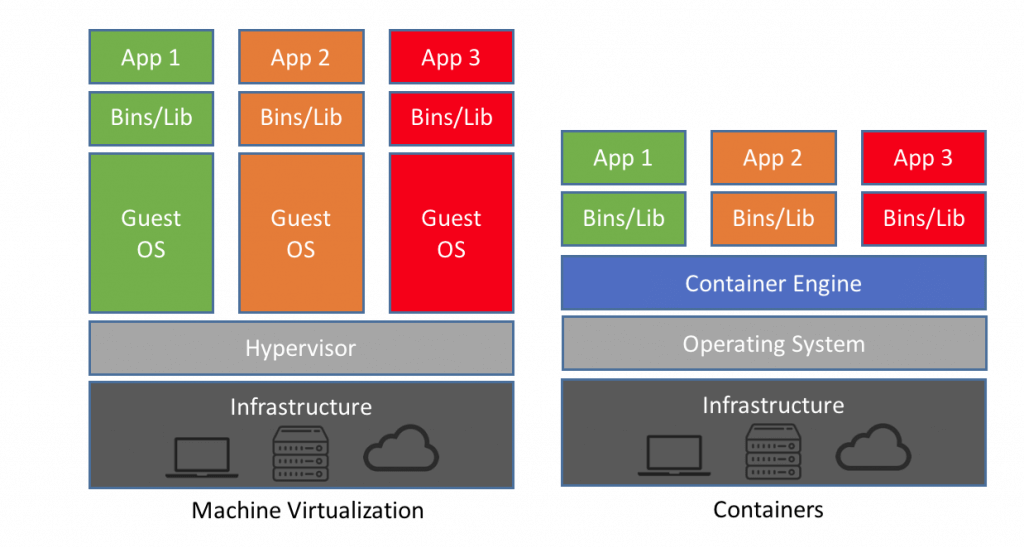
\includegraphics[width=\columnwidth, height=0.5\textheight]{./png/container}
			}%
			\only<2>{%
				\centering Container inside Pod
				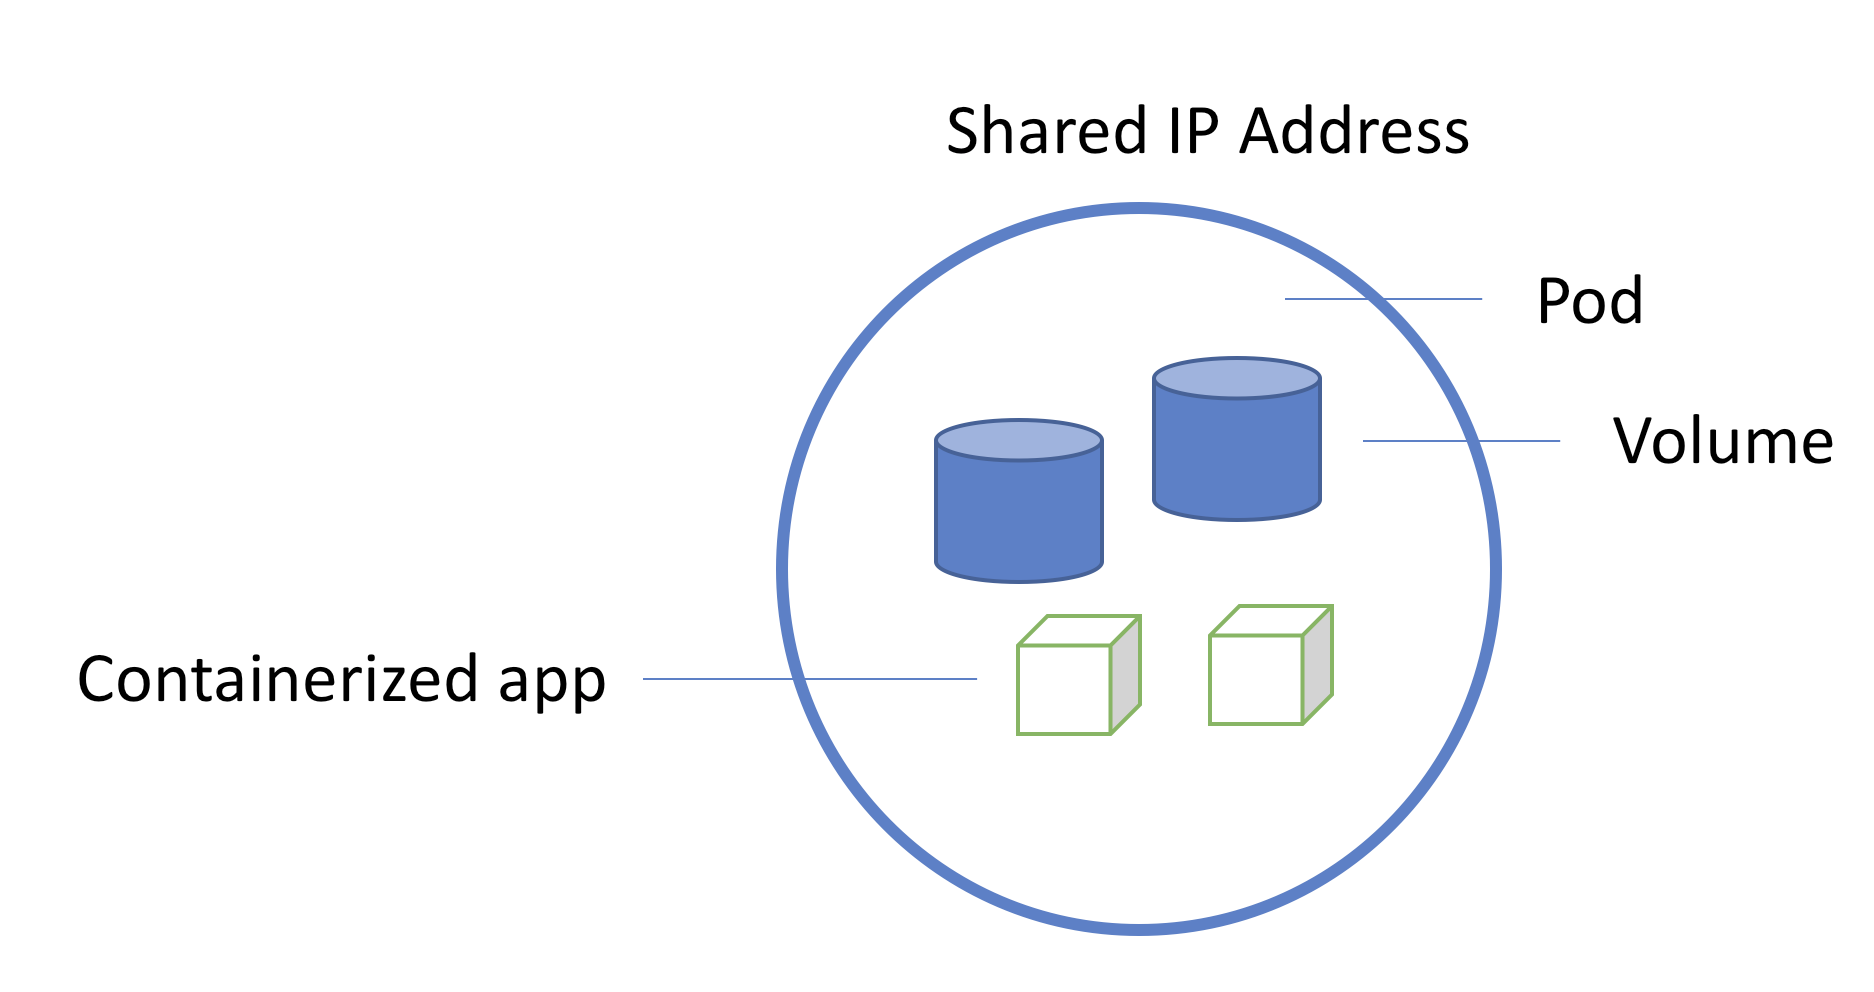
\includegraphics[width=\columnwidth, height=0.5\textheight]{./png/pod}
			}%
			\only<3>{%
				\centering Container Runtime Interface
				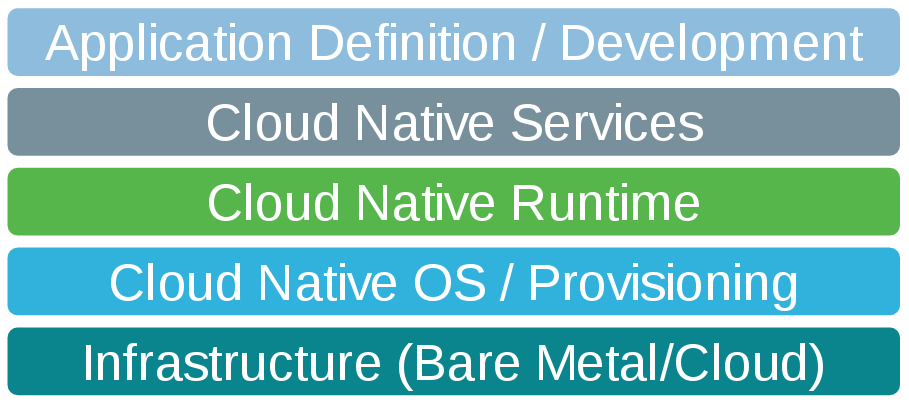
\includegraphics[width=\columnwidth, height=0.5\textheight]{./png/cri}
			}%
			\only<4>{%
				\centering Most known (insecure) socket
				
\includegraphics[width=\columnwidth, height=0.5\textheight]{./png/docker}
			}%
			\only<5>{%
				\centering Most unknown (secure) socket
				
\includegraphics[width=\columnwidth, height=0.5\textheight]{./png/buildah-podman}
			}%
			\only<6>{%
				\centering Lightest fastest socket
				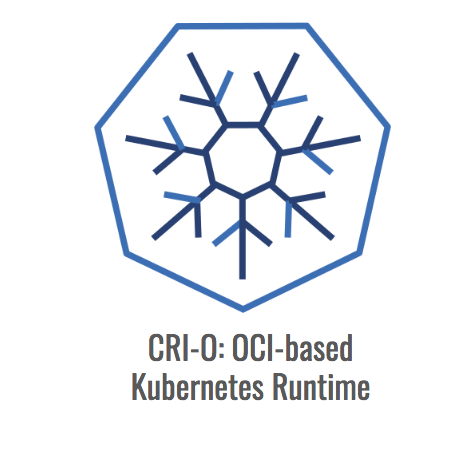
\includegraphics[width=\columnwidth, height=0.5\textheight]{./png/crio}
			}%
			\only<7>{%
				\centering Read about it
				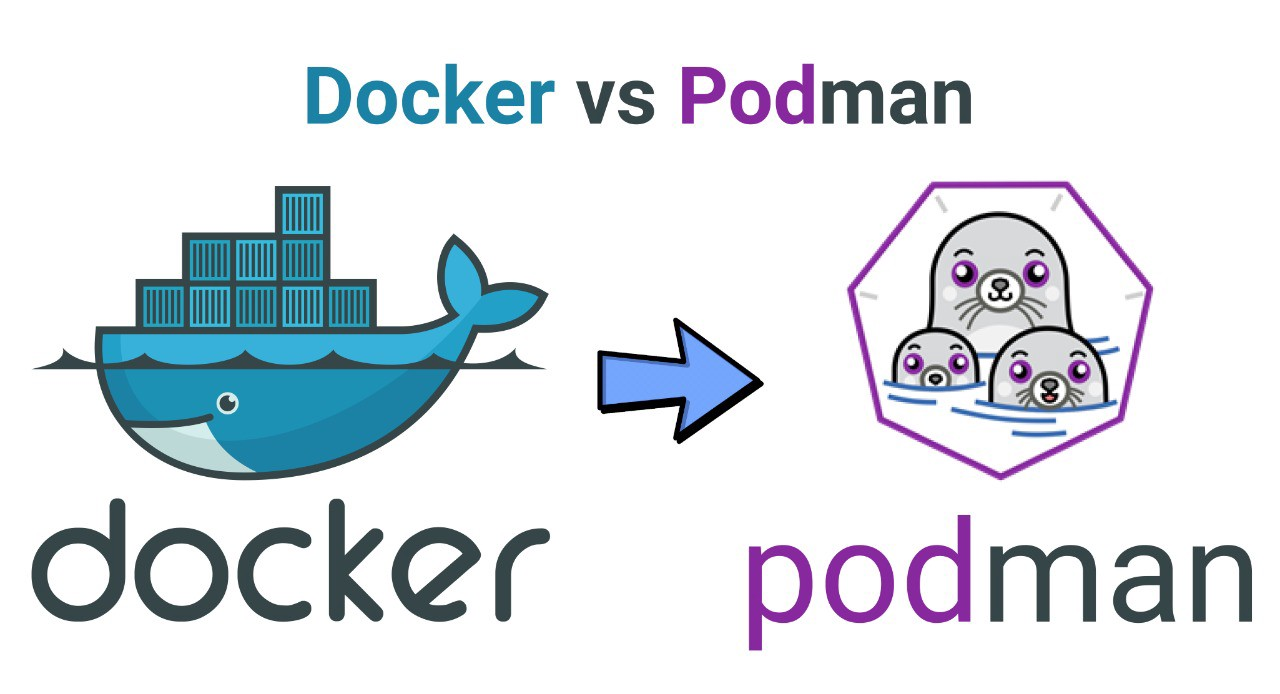
\includegraphics[width=\columnwidth, height=0.5\textheight]{./png/dockervspodman}
			}%
			\only<8>{%
				\centering Is a puzzle of elements
				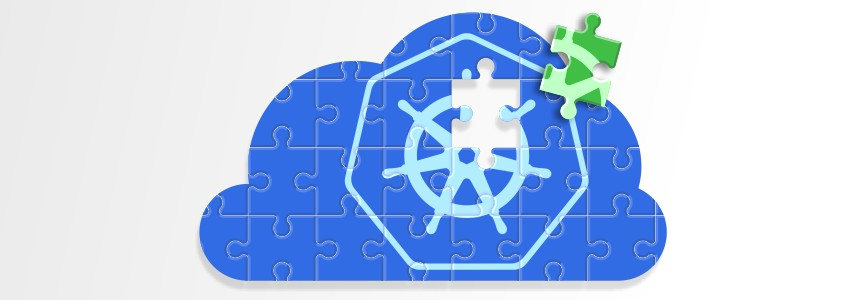
\includegraphics[width=\columnwidth, height=0.5\textheight]{./png/k8sPuzzle.jpg}
			}%
			\caption{k8s Overview} \label{fig:largeFigure}
		\end{figure}
		\end{column}
	\end{columns}
\end{frame}
